\chapter{Estado del arte}

\label{ch:background}

\section{Rayos cósmicos primarios}

Los rayos cósmicos (CR) fueron identificados por primera vez en 1912 por Victor Hess. Hess encontró que la radiación aumentaba considerablemente con la altura y concluyó que tenía origen extraterrestre. Los CR primarios son partículas que viajan a través del espacio hasta interactuar con la atmósfera terrestre generando cascadas de partículas secundarias.\\

El flujo de primarios que llega a la Tierra son 90$\%$ protones, 9$\%$ núcleos de helio y 1$\%$ iones pesados, electrones y otros \cite{Spurio2015}. El origen de los RC primarios depende de su energía, $E$. La mayoría de los CR con $E<10^{10}$ eV provienen del viento solar, para energías $10^{10}$ eV $ < E <$ $10^{18}$ eV el origen más probable es galáctico, en particular de remanentes de supernovas y para $E>10^{18}$ eV la fuente es extragaláctica \cite{Procureur2018}. Recientemente, el observatorio Pierre Auger confirmó que los CR de Ultra Alta Energía (UHECR por sus siglas en inglés) ($> 10^{18}$ eV) proceden de fuera de nuestra galaxia \cite{Pierre2017}.\\

El espectro, $\Phi$, de los CR que ingresan a nuestro planeta se representa con la ley de potencia:

\begin{equation}
  \frac{d \Phi}{dE}  = A \cdot E^{- \alpha} 
\end{equation}
donde $A$ es la normalización respecto al eje \textit{y} y $\alpha$ es el índice espectral diferencial. 
Usualmente el flujo es multiplicado por una potencia de energía, $E^\beta$, para evidenciar ciertas estructuras en el espectro que marcan puntos importantes en el entendimiento del origen de los CR.

\begin{equation}
E^\beta \cdot \frac{d \Phi}{dE}  =   A \cdot E^{- \alpha + \beta}
\end{equation}

\begin{figure}[h!]
\begin{center}
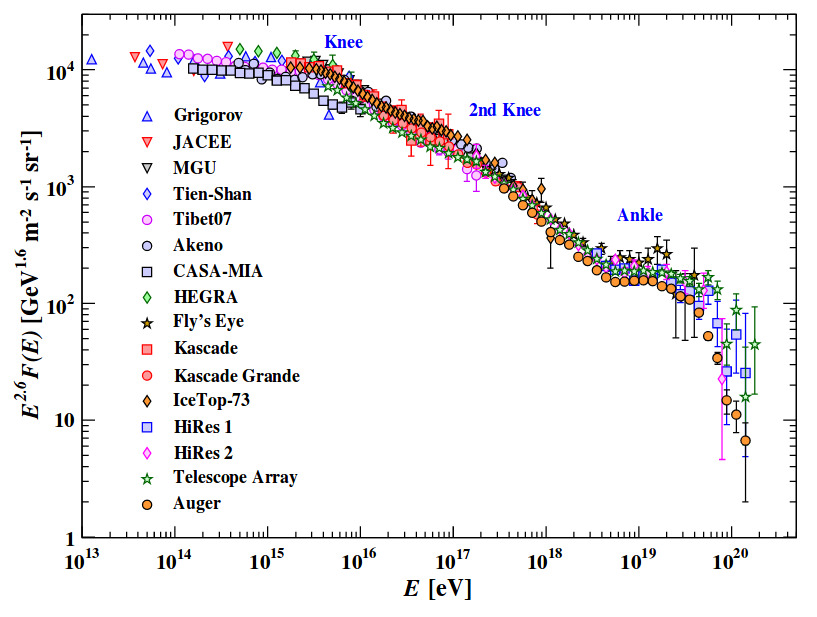
\includegraphics[width=0.9\textwidth]{Figures/Flux}
\caption[Flujo diferencial de CR en función de la energía.]{Flujo diferencial de CR en función de la energía. Los datos de flujo son obtenidos de manera directa o de indirecta por diferentes observatorios (izquierda). Para resaltar las estructuras de la \textit{rodilla} y el \textit{tobillo} se toma un $\beta = 2.6$ \cite{Spurio2015}.}
\label{Flux}
\end{center}
\end{figure}

La caracterización del espectro del flujo de CR se realiza mediante mediciones hechas por diferentes experimentos como se muestra en la Fig. \ref{Flux}. En el espectro se pueden observar dos estructuras particulares asociadas con los cambios de pendiente del espectro. La llamada \textit{rodilla}, alrededor de $10^{15}$ eV, representa una transición entre diferentes clases de mecanismos galácticos de aceleración de CR y de la capacidad de aceleración de las fuentes galácticas. Por otra parte, existe un punto de cambio de pendiente llamado \textit{tobillo} ($\sim 10^{18}$ eV) a partir del cual comienza el flujo de CR de origen extragaláctico, \cite{Spurio2015}.

\section{Partículas secundarias}

Cuando los CR entran a la atmósfera terrestre iteractúan con los núcleos que la componen, produciendo gran cantidad de partículas secundarias (bariones, mesones y leptones). Dependiendo de su tiempo de vida estas partículas pueden interactuar nuevamente o decaer, y generan un efecto cascada llamada lluvia aérea extendida (EAS por sus siglas en inglés). Particularmente, los mesones cargados, típicamente piones y kaones, pueden decaer en muones, electrones y neutrinos, y los piones neutros decaen en fotones.

\begin{figure}[h!]
\begin{center}
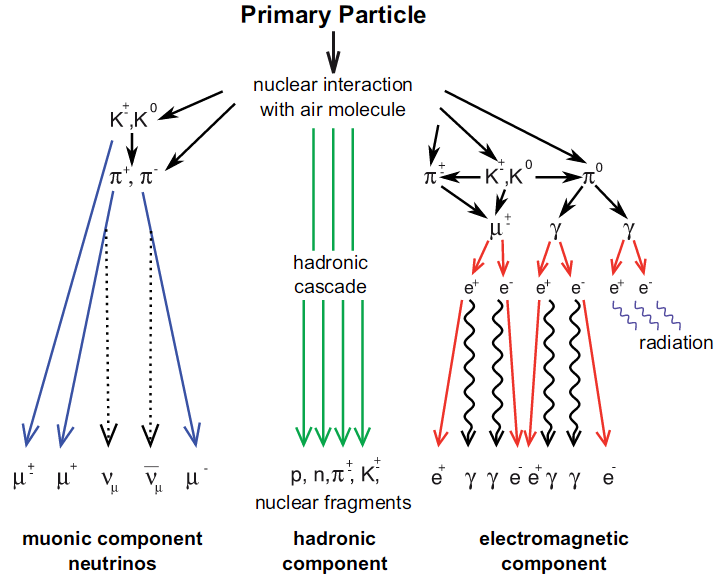
\includegraphics[width=0.7\textwidth]{Figures/EAS_Components}
\caption[Componentes de la lluvia aérea extendida]{La interacción del CR primario con los átomos de la atmósfera genera un chubasco de partículas secundarias compuesto por una parte hadrónica (verde), una electromagnética (roja) y una muónica (azul\textbf{}), \cite{Haungs2011}.}
\label{Components}
\end{center}
\end{figure}

Las EAS tienen tres componentes: la \textbf{electromagnética}, compuesta por fotones, electrones, positrones y usualmente neutrinos electrónicos, la \textbf{hadrónica} compuesta por kaones, piones, neutrones y protones y la componente \textbf{muónica} compuesta por muones y neutrinos muónicos, Fig. \ref{Components}.

El desarrollo longitudinal y lateral de la EAS depende de la energía del CR primario que la genera como se muestra en la Fig. \ref{EAS}. Además, el número total de partículas generado en una EAS se relaciona con el ángulo de incidencia del primario y la altura a la cual ocurrió la primera interacción \cite{Grieder2010}.

\begin{figure}[h!]
\begin{center}
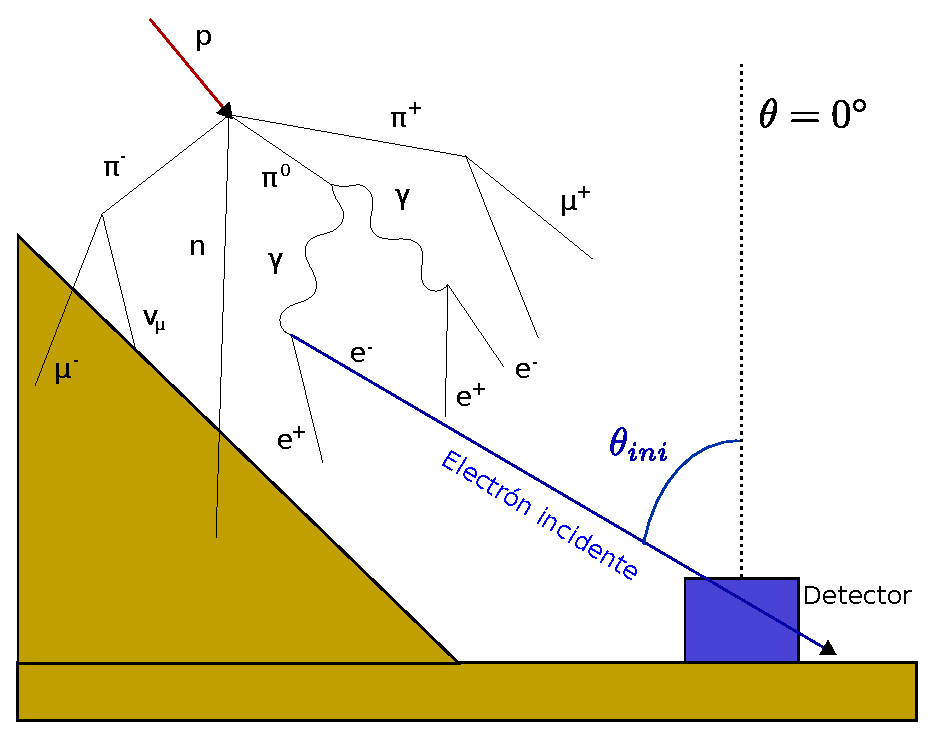
\includegraphics[width=0.5\textwidth]{Figures/EAS}
\caption[Desarrollo longitudinal de una EAS en la atmósfera]{Desarrollo longitudinal de una EAS en la atmósfera. En este caso, se muestra el tamaño de la lluvia en función de la profundidad atmosférica, $X$, para diferentes energías del primario ($E_1<E_2<E_3<E_4$) \cite{Grieder2010}. La profundidad atmosférica se define como la integral en la dirección del primario de la densidad atmosférica sobre el punto de observación.}
\label{EAS}
\end{center}
\end{figure}

\section{Componente muónica}

Las dos fuentes principales de producción de muones corresponden al decaimiento de los kaones $K^{\pm}$ y los piones $\pi^{\pm}$. En el caso de los kaones $K^+$, aproximadamente el $90\%$ de decaimientos ocurre en tres canales \cite{Olive2014}:
\begin{equation}
\begin{array}{ll}
K^+ \rightarrow \mu^+ + \nu_{\mu} & 63.56\% \\
K^+ \rightarrow \pi^+ + \pi^0 & 20.67\% \\
K^+ \rightarrow \pi^+ + \pi^+ + \pi^- &5.58\%
\end{array}
\end{equation}

Para los piones $\pi^\pm$ el $99.9\%$ de los decaimientos ocurren en el canal \cite{Olive2014}:
\begin{eqnarray}
\pi^+ \rightarrow \mu^+ + \nu_{\mu}\\
\pi^- \rightarrow \mu^- + \bar{\nu}_{\mu}
\end{eqnarray}
La componente muónica es la más penetrante de las tres y puede sobrevivir hasta alcanzar la superficie terrestre, debido a dos factores:

\begin{itemize}
\item Un tiempo de vida de $2.2 \times 10^{-6}$ s, el cual es dos órdenes de magnitud mayor a los mesones  $\pi^{\pm}$ $(2.6 \times 10^{-8}$ s) o los $K^{\pm}$ $(1.23 \times 10^{-8}$ s). Debido a su alta energía, los muones pueden desplazarse grandes distancias en la atmósfera sin decaer, $L($km$) = 6200\times E($TeV), \cite{Procureur2018, Nagamine2003}. 

\item Una masa de 105.5 MeV/c$^2$ la cual es $\approx200$ veces mayor que la del electrón. La pérdida de energía por \textit{Bremsstrahlung} es proporcional a $1/m^2$, siendo menor para muones que para electrones a una energía dada. Los muones pierden energía mayormente por ionización hasta energías del orden de 1 TeV en el aire \cite{Groom2001}.

\end{itemize}
